%% Los cap'itulos inician con \chapter{T'itulo}, estos aparecen numerados y
%% se incluyen en el 'indice general.
%%
%% Recuerda que aqu'i ya puedes escribir acentos como: 'a, 'e, 'i, etc.
%% La letra n con tilde es: 'n.
\chapter*{Planteamiento del problema}
\addcontentsline{toc}{chapter}{Planteamiento del problema}
\section*{Marco te'orico}
\addcontentsline{toc}{section}{Marco te'orico}
\subsection*{Cloud computing}
\addcontentsline{toc}{subsection}{Cloud computing}


El c'omputo en la nube es una tecnolog'ia emergente, la cual est'a compuesta por un grupo de recursos heterog'eneos que proveen servicios a trav'es de internet. \cite{agarwal2014efficient} 
Esta tecnolog'ia permite a los consumidores y negocios utilizar aplicaciones sin necesidad de instalaci'on y con acceso a sus archivos personales en cualquier computadora con acceso a internet. \cite{ahmed2012advanced}. 
El c'omputo en la nube se puede clasificar de dos maneras:
\begin{itemize}
\item Por la ubicaci'on: \cite{ahmed2012advanced}  
	\begin{itemize}
	\item \textbf{Nube P'ublica:} La infraestructura de c'omputo se puede compartir entre cualquier organizaci'on.
	\item \textbf{Nube Privada:} La infraestructura de c'omputo es dedicata a una organizaci'on en particular y no se comparte con otras organizaciones.
	\item \textbf{Nube H'ibrida:} Las organizaciones pueden albergar sus aplicaciones cr'iticas en nubes privadas y las aplicaciones con menos problemas de seguridad las puede albergar en nubes p'ublicas.
	\end{itemize}
\item Por el tipo de servicios ofrecidos: \cite{agarwal2014efficient}
	\begin{itemize}
	\item \textbf{Infrastructure as a Service (IaaS):} En 'este nivel, la infraestructura se ofrece como servicio hacia los solicitantes en forma de M'aquinas Virtuales (VM).
	\item \textbf{Platform as a Service (PaaS):} Es una plataforma de desarrollo de aplicaciones que se provee como servicio hacia los desarrolladores para crear aplicaciones basadas en web.
	\item \textbf{Software as a Service (SaaS):} En 'este nivel el proveedor en la nube provee las aplicaciones de software.
	\end{itemize}
\end{itemize}



%%%%%
%%%%%%%%% INSERTAR IMAGEN DEL DRIVE AQUI!
\begin{figure}
	\caption{Esquema general del C'omputo en la Nube}
	\centering
	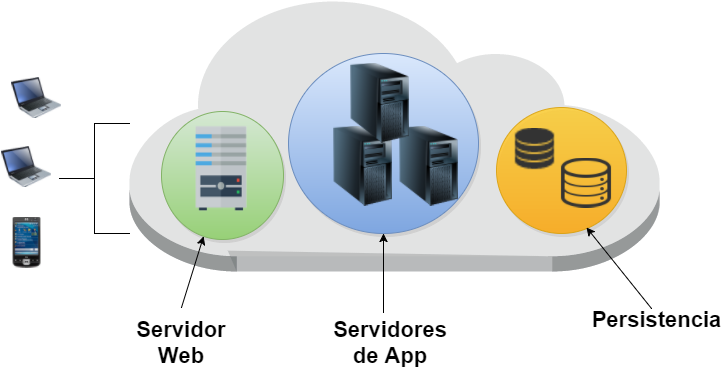
\includegraphics[scale=0.5]{media/cloud1}
\end{figure}
\subsection*{Centro de Datos}
\addcontentsline{toc}{subsection}{Centro de Datos}
Un centro de datos (datacenter) es un espacio dedicado donde las organizaciones almacenan y operan la mayor'ia de su informaci'on y la infraestructura de las tecnolog'ias de comunicaciones que respaldan sus negocios.\cite{whatisdatacenter}

\subsection*{Esquemas de Distribuci'on de Trabajos}
\addcontentsline{toc}{subsection}{Esquemas de Distribuci'on de Trabajos}

La distribuci'on de trabajo (calendarizaci'on) es uno de los puntos principales adem'as de los m'as retadores problemas en el c'omputo en la nube\cite{li2014greedy}. Esta consiste en un conjunto de pol'iticas para controlar el orden en el cual los procesos ser'an ejecutados por el sistema \cite{agarwal2014efficient}.

Existen varios tipos de algoritmos de calendarizaci'on, su principal ventaja es obtener un alto rendimiento al cumplir con las trabajos. Los principales ejemplos de algoritmos de calendarizaci'on son \cite{salot2013survey}:

\begin{itemize}
\item \textbf{FCFS (First Come First Serve) Algorithm:} significa que el trabajo que llegue primero ser'a el primero en ser ejecutado.
\item \textbf{Round Robin Algorithm:} consiste en agregar un tiempo de ejecuci'on para cada trabajo, si dicho tiempo se agota y el trabajo actual no ha finalizado, pasa a un estado de espera y contin'ua con el siguiente trabajo, al finalizar el 'ultimo trabajo regresa a revisar si existen trabajos en espera para proceder a ejecutarlas. 
\item  \textbf{Min-Min Algorithm:} se va ejecutando una por una iniciando por los trabajos de menor tamaño.
\item  \textbf{Max-Min Algorithm:} se va ejecutando una por una iniciando por los trabajos de mayor tamaño.
\item  \textbf{Most fit task scheduling algorithm:} este algoritmo busca los elementos m'as aptos en la cola de trabajos para ejecutarlo primero. Tiene un alto r'adio de error.
\item Priority scheduling algorithm : la idea b'asica es que a cada proceso se le asigna una prioridad, y dependiendo a las prioridades de los dem'as procesos es c'omo se ejecutar'an cada uno de ellos.
\end{itemize}

\subsection*{Balanceo de Cargas}
\addcontentsline{toc}{subsection}{Balanceo de Cargas}

Dentro de nuestro entorno en la nube cada host tiene recursos de hardware finitos y son susceptibles a fallos. Para mitigar contra las fallas y el exhaustivo uso de los recursos, los host son agrupados en clusters, los cuales son esencialmente un agrupamiento de recursos compartidos. El administrador (manager) es capaz de asegurarse que ninguno de los host dentro del cluster es responsable de todas las m'aquinas virtuales dentro de ese cluster \cite{redhat}.

Un entorno de virtualizaci'on responde a los cambios en la demanda para los recursos en cada host haciendo uso del balanceo de cargas, calendarizaci'on de trabajos y migraci'on.

Una pol'itica de balanceo de cargas es configurada para un cluster, que a su vez contiene multiples hosts, cada uno de ellos con distintos recursos de hardware y disponibilidad de memoria. \cite{redhat}
Existen tres pol'iticas para el balanceo de cargas:
\begin{itemize}
\item Sin Balanceo.
\item Distribuci'on Uniforme.
\item Ahorro de Energ'ia.
\end{itemize}

\subsection*{Migraci'on}
\addcontentsline{toc}{subsection}{Migraci'on}

La migraci'on se utiliza para hacer cumplir las pol'iticas dentro del balanceo de cargas. La migraci'on de una m'aquina virtual toma lugar de acuerdo a las pol'iticas de balanceo de cargas para un cluster y la demanda actual sobre los hosts dentro de dicho cluster. La migraci'on de igual manera puede ser configurada para ocurrir autom'aticamente cuando un host es bloqueado o movido a modo de mantenimiento \cite{redhat}. 

\subsection*{Sistemas ERP}
\addcontentsline{toc}{subsection}{Sistemas ERP}

La sigla ERP, en ingl'es Enterprise Resource Planning, significa Planificaci'on de los Recursos de la Empresa. Un sistema ERP constituye un marco de trabajo que incluye aplicaciones comerciales, administrativas (finanzas, contabilidad), recursos humanos, planeamiento de manufactura y gesti'on de proyectos. \cite{saroka2002sistemas}


\section*{Antecedentes}
\addcontentsline{toc}{section}{Antecedentes}

El c'omputo en la nube es una tecnolog'ia que ha abarcado gran parte de los negocios  para dar soporte a ellos. Ésta tecnolog'ia provee a los negocios una ventaja competitiva en los costos de recursos como se ve en los negocios tradicionales, adem'as de la versatilidad que provee al ajustarse a la necesidad de las empresas. \cite{srinivasan2014cloud}

La tecnolog'ia en la nube ha desarrollado una infraestructura fuerte despu'es del surgimiento del c'omputo distribuido.\cite{chen2009cloud} Para obtener las ventajas de dicha tecnolog'ia los usuarios simplemente necesitar'an conectarse a internet y de esta manera tendr'an el acceso al procesamiento de manera remota.\cite{aranganathan2011aco} Sin embargo, para aprovechar el m'aximo potencial de 'estos recursos, es necesario tener en consideraci'on algunas variables,ya que en un entorno en la nube existe un comportamiento din'amico de los recursos a manera que se les provea a los usuarios el servicio.\cite{shimpy2014different}
Una de las pr'acticas con mayor importancia en la nube es la calendarizaci'on, ya que tiene como objetivo administrar las tareas del centro de datos para optimizar los recursos del mismo. De esta manera la eficiencia de la carga de trabajo en la nube aumenta.\cite{shimpy2014different}
En general, el objetivo de la calendarizaci'on en la nube es utilizar los recursos de manera apropiada, mientras la carga de trabajo es distribuida uniformemente para mejorar los tiempos de ejecuci'on.\cite{shimpy2014different}

Debido a la atenci'on que se tiene en la tecnolog'ia en la nube, los centros de datos han tomado un papel muy importante para los servicios empresariales.\cite{shimpy2014different} Un centro de datos est'a compuesto por miles de servidores virtuales ejecut'andose en una instancia de tiempo alojando muchas tareas, al mismo tiempo el centro de datos recibe miles de peticiones a esas tareas. Es aqu'i en donde la programaci'on de trabajos tiene un rol demasiado importante para el c'omputo en la nube, ya que influye en el rendimiento del mismo.\cite{srinivasan2014cloud} 

El problema de la calendarizaci'on pertenece a los algoritmos NP-Dif'icil, lo cual tiene un amplio rango de soluciones posibles y se toma mucho m'as tiempo de encontrar una respuesta ‘optima, ya que no existe un m'etodo para resolver estas inc'ognitas. Sin embargo, es posible estar cerca de la mejor soluci'on contemplando algunos entornos.\cite{shimpy2014different}

\section*{Situaci'on actual}
\addcontentsline{toc}{section}{Situaci'on actual}

Actualmente, hay un mayor n'umero de organizaciones que utilizan el c'omputo en la nube, ya que trae beneficios en cuanto a gastos y recursos. Ya no hay necesidad de invertir tanto en la administraci'on de TI (Information Technology) y existe una mejor capacidad de almacenamiento para los recursos que el 'ambito empresarial necesita.
El c'omputo en la nube utiliza los servicios SaaS (Software as a Service) y HaaS (Hardware as a Service) para hacer m'as eficiente y flexible el uso de la infraestructura de la nube. \cite{mariscal2013computo}

M'exico utiliza, en cuanto a la infraestructura, los servicios ofrecidos por Amazon, Google y Triada (TELMEX). Estos proporcionan almacenaje de informaci'on virtual, plataformas de hospedaje de aplicaciones y servicios en l'inea.\cite{mariscal2013computo} 

Al proveer el servicio se tiene dos escenarios diferentes: cuando hay una mayor demanda de recursos y cuando no la hay,  eso va dependiendo de las necesidades de las empresas. 
Para que se tenga una mejor eficacia durante los servicios, se tiene que mejorar el uso de los recursos en el centro de datos. Dentro del centro de datos hay muchos servidores virtuales que est'an recibiendo trabajos, mientras la nube las mantiene en los lotes de solicitud de trabajos. Es aqu'i, donde resaltamos la importancia de la distribuci'on de trabajos dentro del centro de datos. \cite{shimpy2014different}

En este momento, la distribuci'on de trabajos es un problema NP- dif'icil, pues que no se ha encontrado una soluci'on 'optima. Sin embargo, existen diferentes propuestas para encontrar una mejor soluci'on, utilizando diferentes esquemas de distribuci'on o dicho de otra forma algoritmos. \cite{shimpy2014different}

Existen una gran variedad de algoritmos utilizados en el problema de distribuci'on de trabajos. Los algoritmos m'as utilizados en las investigaciones son: FCFS, Round Robin, Min-Min, Max-Min y Metaheur'istica. Cabe mencionar que en las investigaciones solo hacen una selecci'on de una serie de algoritmos para que, por medio de pruebas, determinen qui'en es el mejor de ellos. 

\section*{Estado del arte}
\addcontentsline{toc}{section}{Estado del arte}

Los siguientes algoritmos de calendarizaci'on actualmente est'an prevaleciendo en la nube:
Resource-Aware-Scheduling Algorithm (RASA) :  Parsa, Entezari-Maleki (2009) proponen el algoritmo RASA, el cual utiliza las ventajas de dos algoritmos tradicionales (Max-min y Min-min) y cubre sus desventajas. Aunque el tiempo limite, la tasa de llegada, costo de ejecucion y costo de comunicaci'on no est'an considerados. \cite{parsa2009rasa}.

\begin{itemize}
\item RSDC (Reliable Scheduling Distributed In Cloud Computing): Delevar, Javanmard, Shabestari y Talebi (2012) proponen un algoritmo confiable en un entorno en la nube, en este algoritmo los trabajos importantes son divididos en sub trabajos, de tal manera que se puedan balancear las peticiones \cite{delavar2012rsdc}.


\item An Optimal Model for Priority based Service Scheduling Policy for Cloud Computing Environment: Dakshayini, Gurupased (2011), proponen un nuevo algoritmo de calendarizaci'on que se basa en la prioridad y un esquema de control de admisi'on. En este algoritmo, la prioridad se asigna a cada proceso admitido en la cola \cite{dakshayini2011optimal}. 


\item Pre-emptable Shortest Job Next Scheduling algorithm (PSJN) :  Este algoritmo se propone en una nube privada. Utiliza la t'ecnica de suscripci'on preferente del algoritmo de Round Robin junto con el siguiente proceso m'as corto (PSN). Brinda beneficios de costos y mejora tiempo de respuesta y tiempo de ejecuci'on \cite{nishant}. 


\item User-priority Guided Min-min scheduling algorithm: Se realiza una mejora para el algoritmo de balanceo de cargas, a trav'es del algoritmo Min-min para la calendarizaci'on de trabajos con el fin de minimizar el tiempo de terminaci'on del ultimo trabajo (makespan) y maximizar la utilizaci'on de los recursos \cite{chen2013user}. 
\end{itemize}

%Existen dos tipos de citas bibliograf'icas: usa \verb|\citep{..}| para
%citas en \emph{par'entesis} y \verb|\citet{..}| para citas
%en el \emph{texto}. Por ejemplo, estudios reciente han mostrado nuevos e
%interesantes modelos que se pueden aplicar para reformular teor'ias
%f'isicas~\citep{NewCam97}. Mientras que, el trabajo de \citet{Rofl06} fue
%considerado muy divertido por una significativa fracci'on de la comunidad
%de investigadores. Tambi'en es posible citar a varios trabajos en una sola
%referencia \citep{Lamport86,Knuth84}.

%Estos comandos para producir citas bibliograficas son provistos por
%el paquete \textsf{natbib}. Para obtener m'as informaci'on, consulta la
%documentaci'on de ese paquete~\citep{doc:natbib}. Por su parte, en
%la documentaci\'on de \textsf{geometry} puedes encontrar detalles
%adicionales sobre el sistema para ajustar los m'argenes del
%documento~\citep{doc:geometry}. Lo que sigue
%es un mont'on de texto sin sentido en lat'in que utilizaremos para llenar
%algunas p'aginas.

